\documentclass[11pt,a4paper,oneside]{scrartcl}
\usepackage[utf8]{inputenc}
\usepackage[english]{babel}
\usepackage{amsmath}
\usepackage{amsfonts}
\usepackage{amssymb}
\usepackage{graphicx}
\usepackage{lmodern}
\usepackage{url}
\usepackage{subfigure}

\usepackage{pgfplots}
\pgfplotsset{compat=newest}
\usepackage{tikz}



\usepackage[lmargin = 2cm,rmargin=2cm, tmargin = 1.8cm,bmargin=2cm]{geometry}

% Listings options
\usepackage{listings}
\usepackage{xcolor}
\definecolor{zebg}{rgb}{1,1,.8} %elfenbeinfarbig

\lstset{language=Matlab, numbers=left, numberstyle=\tiny, basicstyle=\footnotesize,showstringspaces=false,%
 numberblanklines=false, frame=single, backgroundcolor=\color{zebg},xleftmargin=0cm, linewidth=1.11\linewidth}



\author{Lars Schiller\qquad E-10 Simulation GmbH}
\title{Simulation of a tennis ball throwing machine}

\begin{document}
\maketitle


\section{Introduction and task description}

We want to calculate the dropping velocity which is needed for a tennis ball to reach a certain point $y_b$ after a certain time $t_f$. In doing so we taking to account the gravity force and the resistance force due to air drag. The following parameters are known:

\begin{center}
\begin{tabular}{cc|cc|cccc|c}
$y_a$ (Pos$_{t=0}$) & $y_b$ (Pos$_{t=1.5}$) & $g$ & $v_w$ & $\rho_T$ & $\rho_L$ & $c_w$ & $r$ & $t_f$\\ \hline
(0,1) & (14,0) & 9.81$\frac{\textnormal{m}}{\textnormal{s}^2}$ & -10$\frac{\textnormal{m}}{\textnormal{s}}$ & $408\frac{\textnormal{kg}}{\textnormal{m}^3}$ & 1.225$\frac{\textnormal{kg}}{\textnormal{m}^3}$ & 0.47 & 0.034\,m & 1.5\,s \\
\end{tabular}.
\end{center}

\begin{figure}[h]
\begin{center}

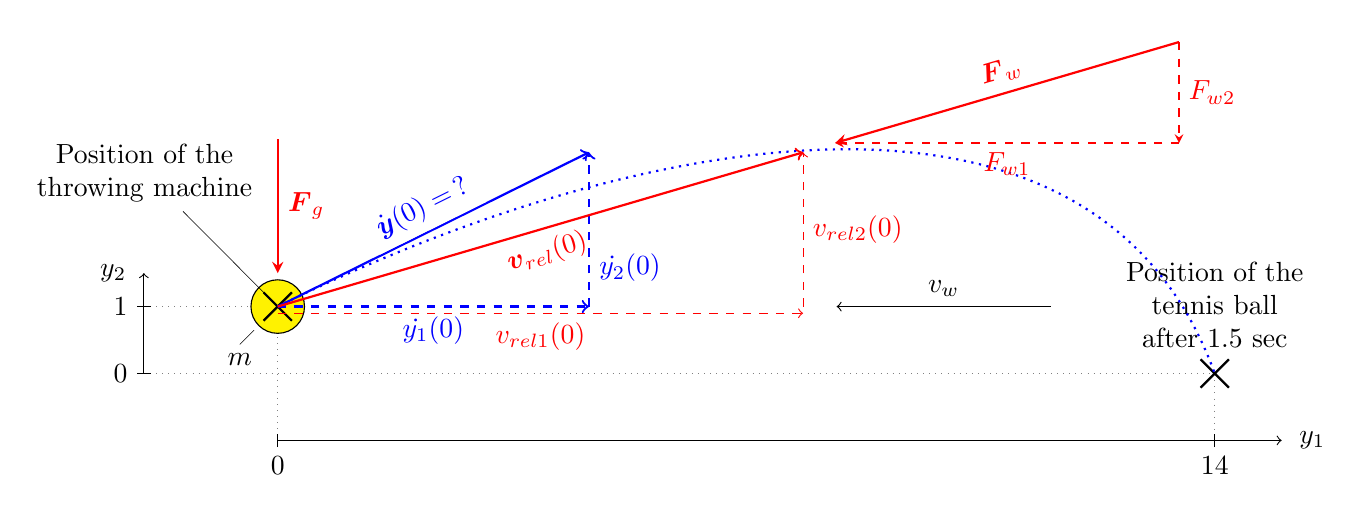
\begin{tikzpicture}[scale = .85]
%% Axis
%\draw[help lines,step = 2] (0,0)grid (15,9);
\draw[help lines,dotted] (-2,1)-|(0,-1);
\draw[help lines,dotted] (-2,0)-|(14,-1);

%% Some values
\def\scale{.32}
\def\yO{7.2*\scale}
\def\xO{14.53*\scale};
\def\vw{-10*\scale};
\def\k{0.08}

\pgfmathsetmacro{\vrel}{sqrt((\xO-\vw)^2 + (\yO)^2)}
\pgfmathsetmacro{\Fx}{\k*\vrel*(\xO-\vw)}
\pgfmathsetmacro{\Fy}{\k*\vrel*(\yO)}
\pgfmathsetmacro{\vabs}{sqrt((\xO)^2 + (\yO)^2)}
\pgfmathsetmacro{\Fabs}{sqrt((\Fx)^2 + (\Fy)^2)}



\draw[->] (0,-1)--(15,-1)node[right=.1cm]{$y_1$};
\draw[->] (-2,0)--(-2,1.5)node[left=.1cm]{$y_2$};
\foreach \x in {0,14}{\draw (\x,-1-.1)node[below]{\x}--(\x,-1+.1);}
\foreach \y in {0,1}{\draw (-2-.1,\y)node[left]{\y}--(-2+.1,\y);}

%% Ball
\draw[fill=yellow] (0,1)circle(.4);
\draw[very thin] (0,1)++(180+45:.5)--++(180+45:.3)node[below]{$m$};

%% Points
\def\w{.3}
\draw [thick] (0,1)+(-45:\w)--+(135:\w) +(225:\w)--+(45:\w);
\path (0,1)++(90:2) node[left=.2cm,align = center,fill = white](A){Position of the \\ throwing machine};
\draw[very thin] (0,1)--(A);
\draw [thick] (14,0)+(-45:\w)--+(135:\w) +(225:\w)--+(45:\w);
\path (14,0) node[above=.2cm,align = center,fill=white]{Position of the \\ tennis ball \\ after 1.5 sec};
%% Trajectory we are looking for
\pgfmathsetmacro{\a}{atan((\yO)/(\xO))}
\path (0,1)coordinate(A);
\draw[dotted,blue,thick] (A)to[out=\a,in=110](14,0)coordinate(B); 
\draw[blue,thick,->] (A)--++(\a:\vabs)node[midway,above,sloped,rectangle,fill=white]{$\dot{\boldsymbol{y}}(0) =\,?$};

\draw[blue,thick,dashed,->] (A)--++(\xO,0)node[midway,below]{$\dot{y_1}(0)$};
\draw[blue,thick,dashed,->] (\xO,1)--++(0,\yO)node[near start,right]{$\dot{y_2}(0)$};


%% Given elements
\draw[->] (\xO-2*\vw+.5,1)--++(\vw,0)node[above,midway]{$v_w$};


%% Elements were are looking for
\draw[thick,red,-stealth] (0,3.5)--++(0,-2)node[right,midway]{$\boldsymbol{F}_g$};

\draw[->,dashed,red] (A)++(0,-.1)--++(\xO-\vw,0)coordinate(X)node[midway,below]{$v_{rel1}(0)$};
\draw[->,dashed,red] (A)++(\xO-\vw,0)--++(0,\yO)coordinate(X)node[midway,right]{$v_{rel2}(0)$};
\draw[->,thick,red] (A)--(X)node[midway,below,sloped]{$\boldsymbol{v}_{rel}(0)$};

\pgfmathsetmacro{\a}{atan((\yO)/(\xO-\vw))}
\draw[thick,stealth-,red] (A)++(\a:\vrel+.5)coordinate(Fi)--++(\a:\Fabs)coordinate(F)node[midway,above,sloped]{$\boldsymbol{F}_w$};
\draw[dashed,red,-stealth] (F)--++(0,-\Fy)coordinate(X)node[right,midway]{$F_{w2}$};
\draw[dashed,red,-stealth] (X)--++(-\Fx,0)node[below,midway]{$F_{w1}$};




\end{tikzpicture}

\caption{principle sketch of the problem to solve}
\label{fig:priciple_sketch}
\end{center}
\end{figure}



\section{Mathematical model of the task}

In order to obtain a system of ordinary differential equations from the given problem one can use \textit{Newtons} 2nd law
\begin{equation}
m\ddot{y} = \sum\limits_i F_i .
\label{eq:newtons2nd}
\end{equation}
It is known, that only the gravity force $\boldsymbol{F}_g$ and the force generated by air drag $\boldsymbol{F}_w$ are applied to the flying ball. 
We can calculate the gravity force to
\begin{equation}
F_g = mg,
\end{equation}
where $m = V \rho_T = \frac{4}{3}\pi r^3 \rho_T $ is the mass of the tennis ball.
We can approximate the drag force with the following approach\footnote{http://www.leifiphysik.de/themenbereiche/reibung-und-fortbewegung}:
\begin{equation}
F_w = k v_{rel}^2 = \frac{1}{2} A_K c_w \rho_L v_{rel}^2,
\label{eq:drag force}
\end{equation}
where $A_K = \pi r^2$ is the cross-sectional area of the ball, $c_w$ is the drag coefficient, $\rho_L$ is the density of the air and $v_{rel}$ the relative velocity of the ball. These forces are illustrated in figure~\ref{fig:priciple_sketch}. With this information we can rewrite equation~\ref{eq:newtons2nd} as:
\begin{equation}
\begin{bmatrix}
\ddot{y}_1 \\ \ddot{y}_2
\end{bmatrix}
= 
\begin{bmatrix}
-\frac{k}{m}\big|v_{rel}\big|\left(\dot{y}_1 -  v_w\right)\\
-\frac{k}{m}|v_{rel}|\dot{y}_2 - g
\end{bmatrix},
\label{eq:2ndode}
\end{equation}
with $|v_{rel}| = \sqrt{\left( \dot{y}_1 -v_w \right)^2 + \dot{y}_2^2}$. 
By defining $y_3 = \dot{y}_1$, $y_4 = \dot{y}_2$ and the state vector $\boldsymbol{y} = [y_1~~ y_2~~ y_3~~ y_4]^T$ we can reformulate equation~\ref{eq:2ndode} to a system of 1st order (non linear) differential equations:
\begin{equation}
\dot{\boldsymbol{y}}
:=  f(\boldsymbol{y}) = 
\begin{bmatrix}
y_3 \\ y_4 \\
-\frac{k}{m}|v_{rel}|\left(y_3-v_w\right)\\
-\frac{k}{m}|v_{rel}|{y_4} - g
\end{bmatrix}.
\label{eq:1stode}
\end{equation}


\section{Choice and description of suited numerical solvers}

Since we are not able to solve boundary value problems (RWP) with the known methods, but 
initial value problems (AWP), the task is to transform this RWP into an AWP.
We already know the the initial value of the first and the second state $\boldsymbol{y}_a = [y_1(0)~~y_2(0)]^T$ and we can guess an initial value for the both other states $\boldsymbol{\eta} = [y_3(0)~~y_4(0)]^T$. We also know the final value of the 1st and 2nd state $\boldsymbol{y}_b = [y_1(t_{f})~~y_2(t_f)]$. With this informations we can set up the residual function $\boldsymbol{F}$: 
\begin{equation}
\boldsymbol{F}(\boldsymbol{\eta}) := \boldsymbol{y}_{\boldsymbol{\eta}}(t_f) - \boldsymbol{y}_b,
\label{eq:F:residuum}
\end{equation}
where $\boldsymbol{y}_{\boldsymbol{\eta}}(t_f)$ is the evaluation at the final time $t_f$ of the solution of the AWP given in equation~\ref{eq:1stode} with the initial condition $\boldsymbol{y}(0)=[\boldsymbol{y}_a ~~ \boldsymbol{\eta}]^T$. If we can find a $\boldsymbol{\eta}$ such that $||\boldsymbol{F}||$ goes to zero, we have found a solution for the RWP.

\subsection{\textit{Newton} - method}
One way for finding a zero of a certain function is the \textit{Newton}-method. We guess an initial $\boldsymbol{\eta}_0$ and calculate the following within a loop while $||\boldsymbol{F}(\boldsymbol{\eta}_k)|| > \texttt{tol}$:
\begin{equation}
\boldsymbol{\eta}_{k+1} = \boldsymbol{\eta}_k - \big( \boldsymbol{JF}(\boldsymbol{\eta}_k) \big)^{-1}\boldsymbol{F}(\boldsymbol{\eta}),
\label{eq:newtonMethod}
\end{equation}
where $\boldsymbol{JF}$ is the Jacobian of $\boldsymbol{F}$. So we have to solve in each iteration step $n+1$ initial value problems, where $n$ is the dimension of $\boldsymbol{F}$ (in this case $n=2$). This is quite expensive.

\subsection{\textit{Broyden} - method}

With a given $\boldsymbol{\eta}_0$ and a given approximation to the Jacobian $\boldsymbol{JF}_0$ we can set up the following iteration loop:
\begin{eqnarray}
\boldsymbol{s}_k &=& - \big(\boldsymbol{JF}_k\big)^{-1}\boldsymbol{F}(\boldsymbol{\eta}_k) \\
\boldsymbol{\eta}_{k+1} &=& \boldsymbol{\eta}_k + \boldsymbol{s}_k \\
\boldsymbol{JF}_{k+1} &=& \boldsymbol{JF}_k + \frac{\boldsymbol{F}(\boldsymbol{\eta}_{k+1}) \boldsymbol{s}_k }{|| \boldsymbol{s}_k ||^2} .
\end{eqnarray}
This is called the \textit{Broyden} - method and needs to solve the initial value problem only once per iteration step, which is much cheaper than \textit{Newton} (eq.~\ref{eq:newtonMethod}).

\subsection{\textit{Dormand} and \textit{Price} method}
To solve the initial value problem the \textit{Dormand} and \textit{Price} method (DOPRI5) is used in both cases \textit{Newton} and \textit{Broyden}. This is an explicit 7-staged \textit{Runge-Kutta} method (RKV) with an order of error $p = 5$ and an embedded step size control. The general form of a RKV looks like :  

\begin{eqnarray*}
\boldsymbol{k}_i &=& f\left(x_n + a_ih_n,\boldsymbol{y}_n+h_n\sum\limits_{j=1}^{i-1}b_{ij}\boldsymbol{k}_j\right)~~(i=1,...,s) \\
\boldsymbol{y}_{n+1} &=& \boldsymbol{y}_n + h_n\sum\limits_{i=1}^sc_i\boldsymbol{k}_i
\end{eqnarray*}
with a \textit{Butcher}-scheme (the values can be looked up in the script p.\,25 )
\begin{tabular}{c|c}
$\boldsymbol{a}$ & $\boldsymbol{B}$  \\ \hline
$p=5$ & $\boldsymbol{c}^T$ \\ \hline
$\hat{p} = 4$ &  $\hat{\boldsymbol{c}}^T$ \\
\end{tabular}.

Now the trick is that there exists a 2nd coefficient vector $\hat{\boldsymbol{c}}$ to the same $\boldsymbol{a}$ and $\boldsymbol{B}$ which results in an order of error $\hat{p} = 4$. So its very cheap to build an error estimator $\varphi$ to control the step size $h_n$ :
\begin{equation}
\varphi = \Bigg| h_n\left(   \sum\limits_{i=1}^sc_i\boldsymbol{k}_i - \sum\limits_{i=1}^s\hat{c}_i\boldsymbol{k}_i \right)\Bigg|
\label{eq:errEstimator}
\end{equation}
So we can increase the step size if $\varphi$ is small and decrease if the estimator exceeds the tolerance.

\section{Description and evaluation of the results}

Figure~\ref{fig:result} illustrates the trajectory of the tennis ball and shows the (scaled) initial velocity $\boldsymbol{\eta}$.
Both methods result in nearly the same outcome. The difference $err = \Big| \boldsymbol{\eta}_{\textnormal{Newton}} - \boldsymbol{\eta}_{\textnormal{Broyden}} \Big| \approx \texttt{1e-5}$  is for practical applications negligible. Another thing to observe is that \textit{Newton} converges a bit faster but needs more total function evaluations.


\begin{figure}[hb]
\centering
\includegraphics[scale=1]{Solution_x14_y.pdf}
\caption{Illustration of the result}
\label{fig:result}
\end{figure}

In table~\ref{tab:eva:results} some statistics of the solving process are listed. It is easy to see that the \textit{Broyden}-method overcomes in almost all categories. And we can expect that if the dimension of the problem and the residual function respectively would be higher, the difference between the total function evaluations and thereby the computational times would be very much larger as well. Since \textit{Newton} needs $n+1$, \textit{Broyden} only 1 solution of the AWP per iteration step.\\
So it is reasonable to prefer the \textit{Broyden}-method to solve the boundary value problem.



\begin{table}[b]
\begin{center}
\begin{tabular}{c|ccc}
method & iteration steps & total fun evals & computational time [sec]\\
\hline
\textit{Newton} & 3 & 1010 & 0.0444 \\
\textit{Broyden} & 4 & 509 & 0.0238 \\

\end{tabular}
\end{center}
\caption{Evaluation of the results}
\label{tab:eva:results}
\end{table}


\end{document} 